\documentclass[11pt, oneside]{article}   	% use "amsart" instead of "article" for AMSLaTeX format
\usepackage{geometry}                		% See geometry.pdf to learn the layout options. There are lots.
\geometry{letterpaper}                   		% ... or a4paper or a5paper or ... 
%\geometry{landscape}                		% Activate for for rotated page geometry
%\usepackage[parfill]{parskip}    		% Activate to begin paragraphs with an empty line rather than an indent
\usepackage{graphicx}				% Use pdf, png, jpg, or eps§ with pdflatex; use eps in DVI mode
								% TeX will automatically convert eps --> pdf in pdflatex		
\usepackage{amssymb}

\title{Ecological model for GEOCLIM: the ECOWEB module}
\author{Yves Godd\'eris}
\date{March 2016}							% Activate to display a given date or no date

\begin{document}
\maketitle


\section{Generality}
%*****************************************************
The model includes three trophic levels: primary producers, predators, and super predators. The ecological model uses the P input in each oceanic reservoir to calculate the uptake of P and C by the primary producers (entrance gate of those elements in the trophic chains). ECOWEB then sends this uptake back to the GEOCLIM model which stores it into the POC reservoir. Within ECOWEB, the exchange fluxes are in molC/yr, and the stocks in molC. Each species is thus represented by a carbon mass.

The number of species of the three trophic levels is fixed prior to any simulation.

\section{Mass balance for the primary producers}
%*****************************************************
At each time step, the mass of species $i$ is calculated by solving the following mass balance equation:
\begin{eqnarray}
%species budget
\frac{dy_{i}}{dt}=\alpha_{i}-\omega_{i}
\label{spbalance}
\end{eqnarray}

where $y_i$ is the biomass of species $i$ (mol C). $\alpha_i$ is the birth rate of species $i$, and $\omega_i$ is the sum of the death rate and grazing rate when applicable.
\subsection{Reproduction rate}
$\alpha_i$ (mol/yr) is dependent on the temperature of the reservoir $T$, on pH, and on the input of dissolved PO$_{4}^{2-}$ inside the oceanic reservoir.
\\
\begin{eqnarray}
%alpha calculation
\alpha_{i}=br_{i} \cdot a_{1}^{i} \cdot \exp{\left[   \frac {-\left(T-b_{1}^{i}\right)^{2}}   {2\left(c_{1}^{i}\right)^{2}}  \right]} \cdot 
         a_{2}^{i} \cdot \exp{\left[   \frac {-\left(pH-b_{2}^{i}\right)^{2}}   {2\left(c_{2}^{i}\right)^{2}}  \right]} \cdot 
        I_{i} \cdot F_{in}^{P}
\label{birth}
\end{eqnarray}

The two exponential factors are gaussian functions. $b_{1}^{i}$ and $b_{2}^{i}$ are respectively the optimum living temperature and pH for the species $i$. $c_{1}^{i}$ and $c_{2}^{i}$ define the temperature and pH tolerance of species $i$. $b_{1}^{i}$ is set to the averaged long term temperature, with a random noise between 0 and $\pm$5 degrees C around the optimum living temperature. The temperature tolerance for each species is randomly set a value between 0 and $\pm$4 degrees C around each respective optimum temperature $b_{1}^{i}$. Optimal living pH $b_{2}^{i}$ and tolerance $c_{2}^{i}$ are similarly randomly set. The interval goes from -0.1 to +0.1 for the noise added to the averaged long term pH of the surficial reservoir. Tolerance runs from $\pm$0.3 pH unit. 

Finally, $I_{i}$ represents the potential competition for resources amongst the primary producers. For each species $i$, the existence of a competitive relationship is randomly fixed (yes/no). If the answer is no, $I_{i,j}$ is set to 1. Conversely, If the answer is yes, $I_{i,j}$ is calculated as follows for species $i$:
\\
\begin{eqnarray}
%competition
I_{i,j}=\frac{\left(\frac{y_i}{y_j}\right)}  {1+\left(\frac{y_i}{y_j}\right)}
\label{competition}
\end{eqnarray}

For species $j$ with respect to species $i$, it is calculated as:
\\
\begin{eqnarray}
%competition
I_{j,i}=1-I_{i,j}
\label{competition2}
\end{eqnarray}

where $y_i$ and $y_j$ are respectively the biomasses of species $i$ and $j$. If the ratio between these two biomasses tends towards 0, then the efficiency of species $j$ in gathering resources leads to the extinction of $i$. If the biomass ratio turns at the advantage of species $i$, and the reproduction of {j) tends towards 0. The factor $I_i$ is calculated as the average of all the $I_i,j$, for $j$ covering the whole range of species in competition with $i$. This formalism implies that if a species is in competition with one or several others, its reproduction rate is somewhat reduced ($I_i$ is little than 1) compared to non-competing species.

\subsection{Death rate}
The death rate of each primary producer is equal to the sum of the natural death rate $D_i$ and the predation rate $G_{i,k}$  of species by the predator $k$ (both fuxes in moleC/year). The death rate is set proportional to the total mass of the primary producer himself:
\\
\begin{eqnarray}
%primary producer death rate
D_i=k_{death} \cdot y_i
\label{death_rate}
\end{eqnarray}

Several predators can feed on the same primary producer species $i$. The is fixed by drawing lots. Then the total loss of biomass of species $i$ due to predation is:
\\
\begin{eqnarray}
%primary producer death rate
G_i=\sum_k {G_(i,k)}=\sum_k {k_{pred}^{k,i} \cdot \frac{\frac{y_i}{y_k}}{10+\frac{y_i}{y_k}} \cdot y_k}
\label{predation_rate}
\end{eqnarray}

where the sum extends over all the predators ($k$) feeding on species $i$. $k_{pred}^{k,i}$ is a fix constant, but can also be randomly fixed. The relative predator biomass within the whole ecosystem depends on this (those) constant(s). The predation rate is also set proportional to the predator biomass (the more they are, the more they eat. But the proportionality is modulated by a Michaelis-Menten function of the prey/predator ratio. Overall, the second term of equation \ref{spbalance} can be written:
\\
\begin{eqnarray}
%species loss
\omega_{i}=D_i + G_i
\label{destruction}
\end{eqnarray}



\section{Mass balance for the predators}
%*****************************************************
The reproduction rate of predators is set to their grazing rate, following the principle that they are tight to the disponibility of ressources. The number of grazed species for each predator is fixed randomly. Some of them are thus specialist (feeding on few species), and other generalist (feeding on many species). Predators are allowed to feed on other predators. This is once again randomly fixed. The death rate of predator is calculated in the same way as the death rate of primary producers.


\section{Mass balance for the super predators}
%***************************************************
Predators of the trophic level 3 behave as predator of the trophic level 2, with the notable exception that they cannot feed on each other. The $D_i$ terms is thus the only term appearing in the calculation of $\omega_i$.

\section{Pelagic carbonate producers}
%***************************************************
A random number of primary producers are assumed to be carbonate shell producers. No more than 20\% of the primary producer species can be carbonate producers (this is an adjustable parameter). For each surficial oceanic reservoir, the ECOWEB module calculates the ratio between the biomass of primary producers building carbonate shells, and the total biomass of primary producers. This ratio is sent to GEOCLIM which translate it into a carbonate flux as a function of the saturation state of the seawater with respect to calcite. Note that if the surface water becomes undersaturated, the carbonate primary producers undergo extinction ($\alpha_i$ is set to zero).


\section{Extinction}
%----------------------
If, for any given reason, the biomass of a species falls below 1\% of its original steady-state value, the species undergoes extinction. $\alpha_i$ is set to zero, translating the fact that the critical threshold below which reproduction is not more possible has been reached. The threshold of 1\% is an adjustable parameter. $\alpha_i$ is maintained to zero even if favorable conditions are restores over the course of the simulation.

%ecoweb scheme
\begin{center}
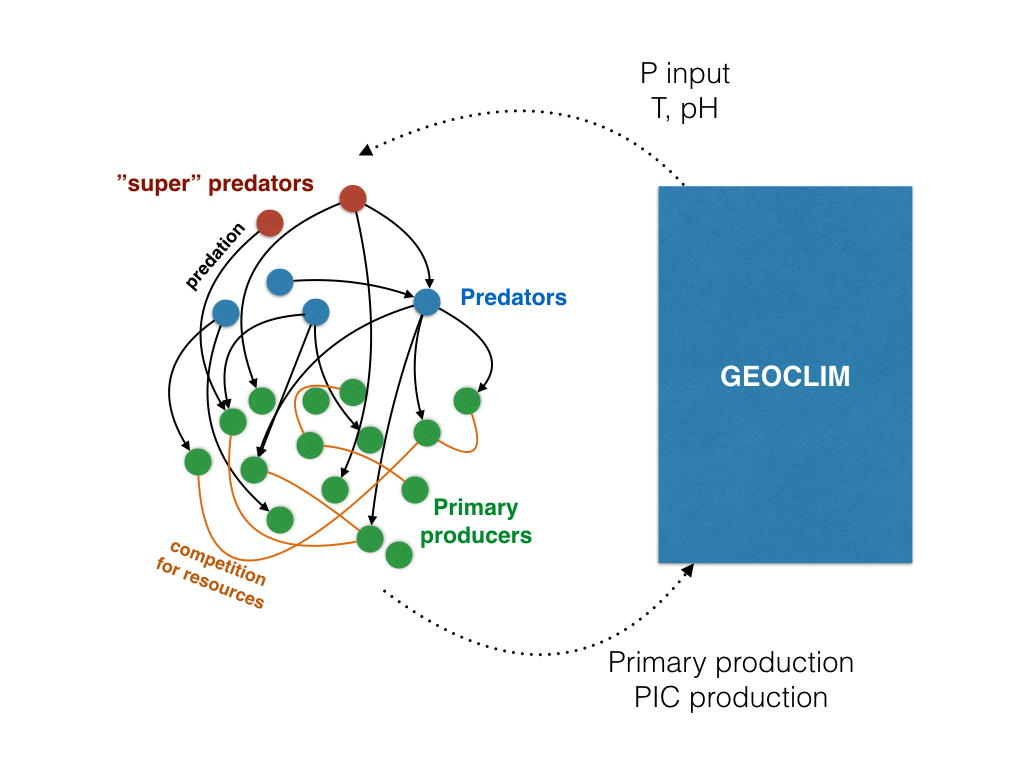
\includegraphics[width=10cm]{/Users/yves/fortran/GEOCLIM2/description/biodiv_scheme.jpg}\\
\small{Schematic view of the ECOWEB module}\\
\end{center}


\end{document}  